\section{Metodo da Bissecao}
%\index{Método da Bisseção}%

\begin{itemize}

\item Características do método
 \begin{itemize}
  \item necessita o intervalo que contém a raiz
  \item não necessita continuidade da derivada de $f(x)$
  \item aplica-se a qualquer tipo de equação, inclusive funções não analíticas
  \item baseado no fato de que quando a raiz de $f(x)$ está em [a,c] os sinais nas duas extremidades mudam: $f(a) \times f(c) \leq 0$ (ver figura \ref{fig:bissecao1}).
 \end{itemize}

\begin{figure}[htb]
  %\index{figura da bisseção}%
  \setlength{\abovecaptionskip}{20pt}
  %%% o valor default de \abovecaptionskip definido para a classe
  %%% article e de 10pt.
  \centering
  %%% VIDE ABAIXO COMENTARIO SOBRE USO DE DIRETORIOS NO PATHNAME
  %%% DOS ARQUIVOS INCLUIDOS.
  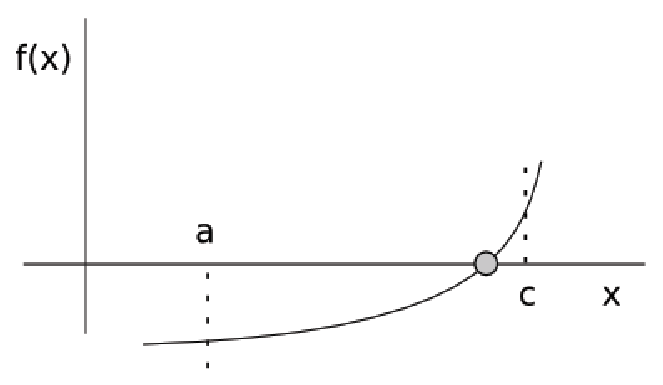
\includegraphics[scale=0.5]{capitulos/capitulo1/figuras/bissecao1.eps}
  \caption{Função $f(x)$ com isolamento [a,c].}
  \label{fig:bissecao1}
\end{figure}

\end{itemize}

\begin{algorithm}{htbp}

  \caption{Método da Bisseção}

  \begin{algorithmic}
    \STATE \textbf{Inicialização:} $i=0$, $a_{0}=a$, $c_{0}=c$

    \STATE \textbf{Iteração i:}

    \begin{enumerate}
     \item tamanho do intervalo, $\displaystyle s_{i} = c_{i}-a_{i} = \frac{s_{0}}{2}^{(i)}$
     \item Se $ \displaystyle \frac{s_{i}}{2} \leq \textit{\textbf{tol}} $

      $ \displaystyle \textit{x}_{i} = \frac{(a_{i} + c_{i})}{2} $

      $ \displaystyle \textit{err}_{i} = \frac{s_{i}}{2} = {\frac{s_{0}}{2}}^{(i+1)} $

      sai

      Se $ \displaystyle \frac{s_{i}}{2} > \textit{\textbf{tol}} $, vá para 3.

      \item Calcule

      $ \displaystyle b_{i} = \frac{(a_{i} + c_{i})}{2} $

      $ f(a_{i}) \ast f(b_{i}) $

      $ f(b_{i}) \ast f(c_{i}) $

      \item Se $ f(a_{i}) \ast f(b_{i}) \leq 0 $, (raiz em [$a_{i}$, $b_{i}$])

      faça $i = i + 1$, $c_{i} = b_{i-1}$, vá para 1.

      Se $ f(b_{i}) \ast f(c_{i}) \leq 0 $, (raiz em [$b_{i}$, $c_{i}$]),

      faça $i = i + 1$, $a_{i} = b_{i-1}$, vá para 1.

    \end{enumerate}

  \end{algorithmic}

\end{algorithm}

\begin{displaymath}
 \frac{c_{0} - a_{0}}{2^{n+1}} \leq \textit{\textbf{tol}}
\end{displaymath}
\begin{displaymath}
 \Rightarrow \frac{c_{0} - a_{0}}{\textit{\textbf{tol}}} \leq 2^{(n+1)}
\end{displaymath}
\begin{displaymath}
 \Rightarrow n + 1 \geq \log_{2}\left( \frac{c_{0}-a_{0}}{\textit{\textbf{tol}}} \right)
 = \frac{ \ln \left( \frac{c_{0}-a_{0}}{\textit{\textbf{tol}}} \right) }{\ln(2)}
\end{displaymath}
\begin{displaymath}
 \Rightarrow n \geq \ln\left( \frac{c_{0}-a_{0}}{ln(2)} - 1 \right)
\end{displaymath}

\textbf{Observações:}

\begin{itemize}
\item após \textbf{n} iterações o tamanho do intervalo é $\displaystyle \frac{(c-a)_{0}}{2^{n}}$

\item o erro máximo na n-ésima iteração é
$\displaystyle \textbf{err}_{n} = \frac{s_{n}}{2} = \frac{s_{0}}{2^{(n+1)}}$

\item Se \textit{\textbf{tol}} é dada, o número de iterações necessárias é dado por
\begin{displaymath}
\displaystyle \frac{c_{0}-a_{0}}{2^{(n+1)}} < \textit{\textbf{tol}}
\end{displaymath}
ou
\begin{displaymath}
n \geq \frac{\ln\left( \frac{c_{0}-a_{0}}{\textit{\textbf{tol}}} \right)}{\ln(2)-1}
\end{displaymath}
\end{itemize}

\begin{example}

\begin{itemize}
\item $ c_{0} - a_{0} = 1$ e $\textit{\textbf{tol}} = 0.0001 $

\item $ n \geq \frac{\ln\left(\frac{1}{0.0001} \right)}{\ln(2)} - 1 = 13.28 - 1 = 12.28 $

\item $n = 13$ ( $14^{a}$ iteração )

\end{itemize}

\end{example}

\begin{example}
 A raiz de $ f(x) = e^{x} - x = 0 $
está no intervalo [0,2]. Encontre uma aproximação da raiz dentro de uma tolerância de 0.01 pelo método da bisseção.

\textbf{Solução:}

\begin{enumerate}
 \item Solução exata: $ e^{x} - 2 = 0 \Rightarrow e^{x} = 2 \Rightarrow x = \ln 2 = 0.6931 $
 \item Solução pelo método da bisseção (ver tabela \ref{tab:bissecao})

\begin{table}[htp]
\footnotesize
	\centering
		
		\begin{tabular}{|c|c|c|c|c|c|c|c|}
		\hline		
		\textbf{Iteração} & \textbf{a} & \textbf{b} & \textbf{c} & \textbf{f(a)} & \textbf{f(b)} & \textbf{f(c)} & \textbf{Erro máximo}\\
		\hline \hline 
		0 & 0 & 1 & 2 & -1 & 0.7182 & 5.3890 & 1\\
		\hline 
		1 & 0 & 0.5 & 1 & -1 & -0.3512 & 0.7182 & 0.5\\
		\hline 
		2 & 0.5 & 0.75 & 1 & -0.3512 & 0.1170 & 0.7182 & 0.25\\
		\hline 
		3 & 0.5 & 0.625 & 0.75 & -0.3512 & -0.1317 & 0.1170 & 0.125\\
		\hline 
		4 & 0.625 & 0.6875 & 0.75 & -0.1317 & -0.0112 & 0.1170 & 0.0625\\
		\hline 
		5 & 0.6875 & 0.7187 & 0.75 & -0.0112 & 0.0518 & 0.1170 & 0.03125\\
		\hline  
		6 & 0.6875 & 0.7031 & 0.7187 & -0.0112 & 0.0200 & 0.0518 & 0.015625\\
		\hline 
		7 & 0.6875 & 0.6953 & 0.7031 & -0.0112 & 0.0043 & 0.0200 & 0.0078125\\
		\hline
		\end{tabular}
	%\caption{Iterações do método da bisseção}
	\caption[Exemplo de iterações do método da bisseção]{A oitava aproximação da raiz é $x = 0.6953$ o máximo erro possível é $0.0078 < 0.01$.}
	\label{tab:bissecao}
\end{table}

\end{enumerate}

\end{example}

\textbf{Notas:}

\begin{enumerate}
 \item O critério $f(a) \ast f(b) \leq 0$ é satisfeito sempre que o número de raízes no intervalo for ímpar. Assim o método encontra uma das raízes (ver figura \ref{fig:bissecao2}).

\begin{figure}[htb]
  %\index{figura da bisseção}%
  \setlength{\abovecaptionskip}{20pt}
  %%% o valor default de \abovecaptionskip definido para a classe
  %%% article e de 10pt.
  \centering
  %%% VIDE ABAIXO COMENTARIO SOBRE USO DE DIRETORIOS NO PATHNAME
  %%% DOS ARQUIVOS INCLUIDOS.
  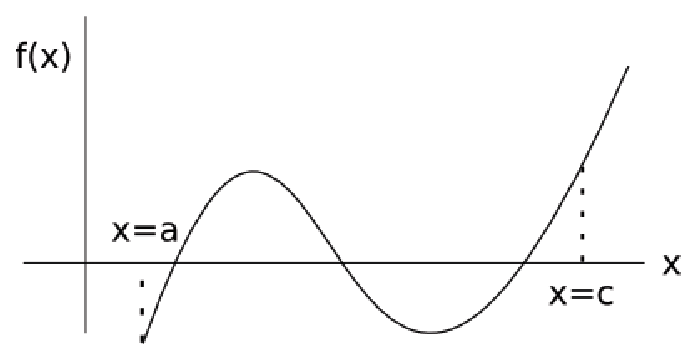
\includegraphics[scale=0.8]{capitulos/capitulo1/figuras/bissecao2.eps}
  \caption{Função $f(x)$ com número de raízes ímpar.}
  \label{fig:bissecao2}
\end{figure}

\item O método da bisseção não pode encontrar um par de raízes duplas porque a função tangencia o eixo x (ver figura \ref{fig:bissecao3}).

\begin{figure}[htb]
  %\index{figura da bisseção}%
  \setlength{\abovecaptionskip}{20pt}
  %%% o valor default de \abovecaptionskip definido para a classe
  %%% article e de 10pt.
  \centering
  %%% VIDE ABAIXO COMENTARIO SOBRE USO DE DIRETORIOS NO PATHNAME
  %%% DOS ARQUIVOS INCLUIDOS.
  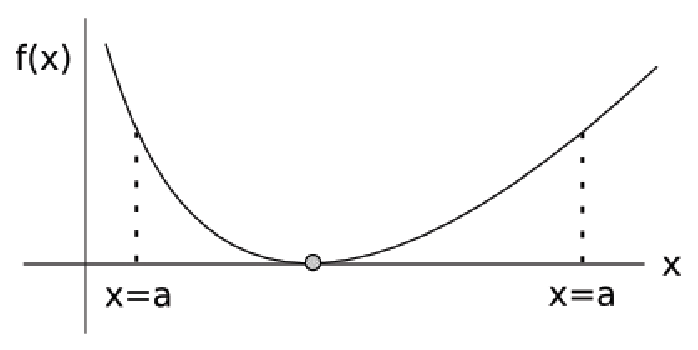
\includegraphics[scale=0.8]{capitulos/capitulo1/figuras/bissecao3.eps}
  \caption{Função $f(x)$ com um par de raízes duplas.}
  \label{fig:bissecao3}
\end{figure}

\item O método pode confundir um ponto de singularidade com uma raiz. Para evitar que isso aconteça, verifique se $|f(c) - f(a)| = 0 $ a medida que o processo avança (ver figura \ref{fig:bissecao4}).

\begin{figure}[htb]
  %\index{figura da bisseção}%
  \setlength{\abovecaptionskip}{20pt}
  %%% o valor default de \abovecaptionskip definido para a classe
  %%% article e de 10pt.
  \centering
  %%% VIDE ABAIXO COMENTARIO SOBRE USO DE DIRETORIOS NO PATHNAME
  %%% DOS ARQUIVOS INCLUIDOS.
  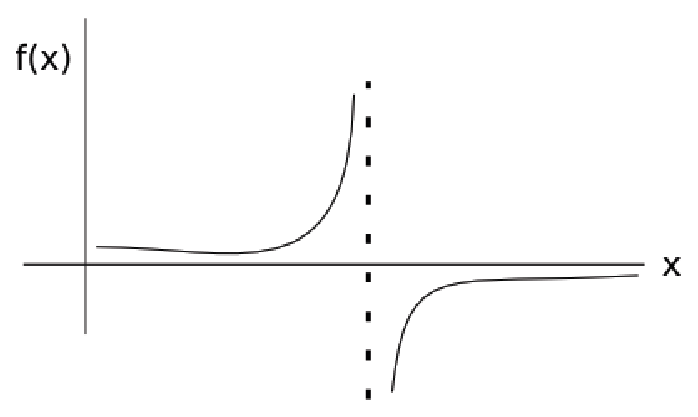
\includegraphics[scale=0.8]{capitulos/capitulo1/figuras/bissecao4.eps}
  \caption{Função $f(x)$ onde pode haver confusão entre ponto de singularidade com uma raiz.}
  \label{fig:bissecao4}
\end{figure}

\item Quando não se tem informação prévia sobre valores aproximados das raízes, uma maneira fácil de encontrar intervalos contendo raízes é imprimir uma tabela da função para valores de x igualmente espaçados ou plotar a função utilizando computação gráfica.

\end{enumerate}

\textbf{Nota falada do professor:}

\begin{itemize}
 \item Antes de iniciar o método deve-se identificar por tabela ou gráfico os intervalos que contêm raízes.

 \item O método encontra a raiz de uma função se a raiz existir no intervalo dado.

 \item O método encontra a raiz de uma função mesmo quando a função não é analítica.

 \item O método não distingue entre uma raiz e um ponto de singularidade.
\end{itemize}